\chapter{Regularized Alternating Least Squares: Flexible Regularization for CCA}
\label{chap:als}
\minitoc

\section{Introduction}\label{sec:introduction}

The content relating to regularised alternating least squares as a method for optimizing regularised CCA is based on an abstract which I presented in poster form at OHBM. The work benefitted from extensive theoretical discussions with John Shawe-Taylor and Janaina Mourao-Miranda as well as Janaina and Rick Adams' help interpreting the results.

Canonical Correlation Analysis (CCA) has been an indispensable tool for discovering relationships between two multivariate sets of variables, commonly referred to as views. However, traditional CCA models often fail to adequately handle high-dimensional data, a challenge that is frequently encountered in brain research. To tackle this issue, we introduce a framework for regularized CCA based on alternating least squares (ALS), termed as Flexible Regularized Alternating Least Squares (FRALS). This work forms an early part of my PhD research and primarily aims to show that 'true CCA' models can unveil stronger signals in brain-behaviour data compared to Partial Least Squares (PLS) models.

\subsection{Problem Statement}\label{subsec:problem-statement}
The classical CCA methodology encounters difficulties when applied to high-dimensional datasets. These challenges include overfitting and the possibility of drawing spurious conclusions. While regularization techniques like ridge or lasso regression have been employed to alleviate these issues, they often lack the flexibility needed to cater to various types of data and research queries.

\subsection{Contributions}\label{subsec:contributions}
Our main contribution is the development and evaluation of FRALS, a novel framework that allows the utilization of any regularized least squares solver. This innovation enhances flexibility and provides a more robust defense against the risk of overfitting. Although our experimental outcomes indicate that FRALS excels in terms of out-of-sample correlation, it is important to note that the algorithm ultimately proves to be too slow and impractical for most applications. Nonetheless, it serves as an instructive stepping stone in the ongoing quest for efficient and reliable CCA methods.

\section{Background}\label{sec:background}

\subsection{Regularized CCA}\label{subsec:regularized-cca}
Traditional approaches to regularized CCA include the use of ridge penalties (RCCA) and sparse methods like Penalized Matrix Decomposition (PMD). These methods each have their own limitations; for example, RCCA does not produce sparse solutions, while PMD may miss low-variance but high-correlation directions.

\section{Methods}\label{sec:methods}

\subsection{Flexible Regularized Alternating Least Squares (FRALS)}\label{subsec:flexible-regularized-alternating-least-squares-(frals)}
We adopt an alternating minimization strategy to solve the CCA problem.
The objective is to minimize the sum of squared Frobenius norms between the latent variables and their projections in each view.
Regularization terms are added to the objective function to avoid overfitting.
Our formulation allows the incorporation of any regularized least squares solver, making it extremely flexible.

\subsubsection{Mathematical Formulation}
We can solve CCA by alternating minimization over each view, based on the alternating least squares form.
This form finds a variable $\bold{T}$ that is close to the latent variables $\bold{X}_i\bold{W}_i$, where $\bold{X}_i$, $\bold{W}_i$ are the matrix and weights for each view $i$.
The closer $\bold{T}$ is to $\bold{X}_i\bold{W}_i$, the higher the correlation between them.
The constraint  $\bold{T^{\top}T}=\bold{I}$ ensures that the latent space is orthogonal to find different effects.

\begin{gather*}
    \underset{\bold{W},\bold{T}}{\mathrm{argmin}}\left\{\sum_i \|\bold{X}_i\bold{W}_i-\bold{T}\|_{F}^2 \right\}\\
    \text{subject to: } \bold{T^{\top}T}=\bold{I}\\
\end{gather*}

To regularize the projection matrices, we add penalty terms to the objective function, such as $P(\bold{W}_i)=\lambda_i\|\bold{W}_i\|_F$ for ridge regression or $P(\bold{W}_i)=\lambda_i\|\bold{W}_i\|_1$ for lasso.
This can help us avoid overfitting and improving the interpretability of the results.
This means that \textbf{any regularized least squares solver} can be used to solve each subproblem, such as ridge regression, lasso, elastic net, etc.\ making our framework substantially more flexible than prior work.

\begin{gather*}
    \underset{\bold{W},\bold{T}}{\mathrm{argmin}}\left\{\sum_i \|\bold{X}_i\bold{W}_i-\bold{T}\|_{F}^2 + \textcolor{red}{\lambda_i P(\bold{W}_i)}\}\right\}\\
    \text{subject to: } \bold{T^{\top}T}=\bold{I}\\
\end{gather*}

\section{Experiments}\label{sec:experiments}

\subsection{Experiment 1: Simulated Data Evaluation}\label{subsec:exp1}

In this experiment, we evaluate several Sparse Canonical Correlation Analysis (CCA) variants using synthetic data generated with the FRALS framework.
Two of these variants, IPLS+ and ElasticNet, are implemented within the FRALS framework for added flexibility.
We provide intuition for the comparison of these models:

- \textbf{IPLS+ (Sparse CCA via Iterative Penalized Least Squares with Positive Constraints):} IPLS+ assumes a prior about the data generation process, specifically that the true weights are positive.
This prior matches the data generation process, making it more suitable for the given synthetic data.
As a result, IPLS+ is expected to perform well as it aligns with the underlying data structure.

- \textbf{ElasticNet:} ElasticNet, another model implemented using the FRALS framework, offers a combination of L1 (lasso) and L2 (ridge) regularization.
While it provides flexibility in handling different types of data, it may not align with the specific prior assumption of positive weights in our synthetic data generation process.

\subsubsection{Simulated Data Generation}\label{subsubsec:simulated-data-generation}

In this experiment, we evaluate several Sparse Canonical Correlation Analysis (CCA) variants using synthetic data generated with the FRALS framework. Two of these variants, IPLS+ and ElasticNet, are implemented within the FRALS framework for added flexibility.

Therefore, we anticipate that IPLS+ may outperform ElasticNet due to its alignment with the prior assumptions about data generation. This experiment aims to validate this intuition by comparing the performance of these models and others.

\subsubsection{Methodology}

To carry out the experiment, we leverage the CCA-Zoo Python package. The synthetic data is generated using the \texttt{LinearSimulatedData} class from the package, with parameters set to emulate a high-dimensional feature space.

\begin{table}[h]
\centering
\caption{Experiment Parameters}
\begin{tabular}{l|l}
\textbf{Parameter} & \textbf{Value} \\
\hline
Number of samples (\textit{n}) & 500 \\
Number of features in View 1 (\textit{p}) & 200 \\
Number of features in View 2 (\textit{q}) & 200 \\
Latent dimensions & 1 \\
Sparsity in View 1 & 0.1 \\
Sparsity in View 2 & 0.1 \\
Target correlation between views & 0.9 \\
\end{tabular}
\label{table:experiment-parameters}
\end{table}

We employ several CCA variants for this experiment:

\begin{table}[h]
\centering
\caption{Employed CCA Variants}
\begin{tabular}{l}
\textbf{CCA Variant} \\
\hline
Canonical Correlation Analysis (CCA) \\
Partial Least Squares (PLS) \\
Sparse CCA via Penalized Majorization-Minimization (SCCA\_PMD) \\
Sparse CCA via Iterative Penalized Least Squares (SCCA\_IPLS) \\
Sparse CCA via Span Regularization (SCCA\_Span) \\
Elastic CCA \\
\end{tabular}
\label{table:cca-variants}
\end{table}

Grid search is used for hyperparameter tuning for Elastic CCA and SCCA\_PMD models.

\subsubsection{Evaluation Metrics}

The models are evaluated based on their correlation score on a validation set comprising 20\% of the original data. Additionally, the weights of each model are visualized for interpretability.

\section{Results and Discussion}

\subsection{Performance Comparison}

\subsection{True Weights for Context}

Figure~\ref{fig:True_weights} provides a ground truth reference for the weights in the true underlying signal, setting the context for our subsequent analysis.

\begin{figure}[h]
    \centering
    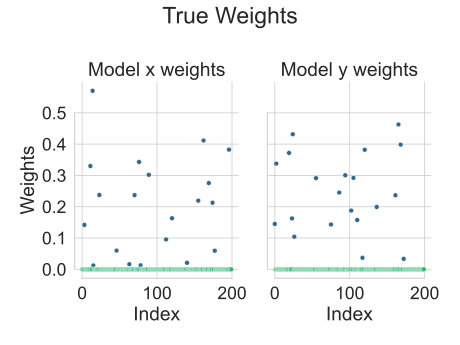
\includegraphics[width=0.6\textwidth]{figures/als/simulated/True_weights.svg}
    \caption{Ground truth weights for the true underlying signal.}
    \label{fig:True_weights}
\end{figure}

\subsection{Interpretation of Weight Plots}

Figures~\ref{fig:CCA_weights} to~\ref{fig:IPLS+_weights} visualize the weights attributed to each feature by different models.
Different colors indicate the indices of weights involved in the true signal (as shown in Figure~\ref{fig:True_weights}) and those not involved.

\subsection{Performance Insights}

\paragraph{Impact of Sparsity:}
Figure~\ref{fig:PLS_weights} and Figure~\ref{fig:CCA_weights} display the weights for PLS and CCA, respectively.
Both models lack sparsity priors and hence select all features with non-zero weights.
This dilutes the true signal and results in lower validation correlation.

\begin{figure}[h]
    \centering
    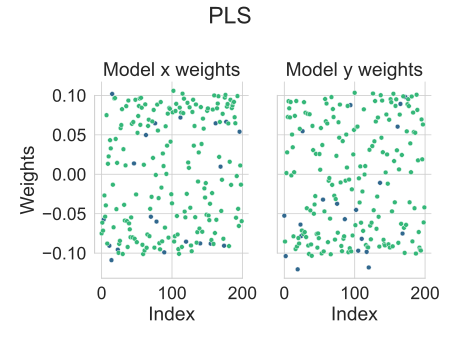
\includegraphics[width=0.6\textwidth]{figures/als/simulated/PLS_weights.svg}
    \caption{PLS selects all features with non-zero weights, leading to diluted true signals.}
    \label{fig:PLS_weights}
\end{figure}

\begin{figure}[h]
    \centering
    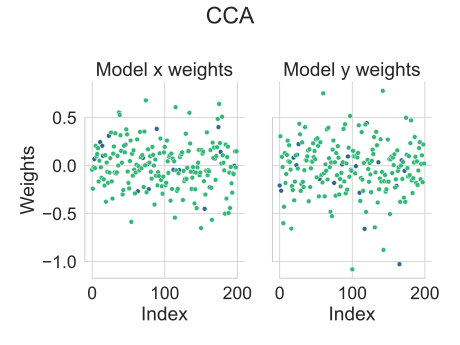
\includegraphics[width=0.6\textwidth]{figures/als/simulated/CCA_weights.svg}
    \caption{ Similar to PLS, CCA also lacks a sparsity prior, leading to poor feature selection.}
    \label{fig:CCA_weights}
\end{figure}

\paragraph{Objective Mismatch:}
In contrast, PMD incorporates a sparsity prior. However, as seen in Figure~\ref{fig:PMD_weights}, its objective is to maximize covariance, not correlation. This leads to its middling performance.

\begin{figure}[h]
    \centering
    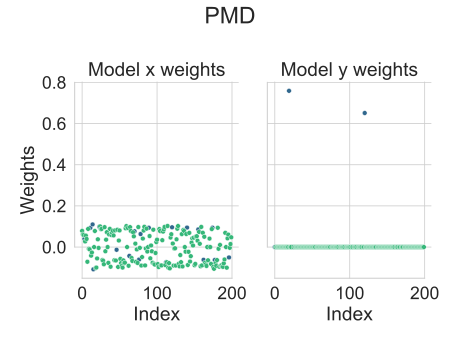
\includegraphics[width=0.6\textwidth]{figures/als/simulated/PMD_weights.svg}
    \caption{PMD shows sparsity but focuses on maximizing covariance rather than correlation.}
    \label{fig:PMD_weights}
\end{figure}

\paragraph{Efficacy of IPLS:}
IPLS performs well due to its alternating lasso procedure and sparsity priors on each view. Figure~\ref{fig:IPLS_weights} confirms its ability to better capture the true underlying signal.

\begin{figure}[h]
    \centering
    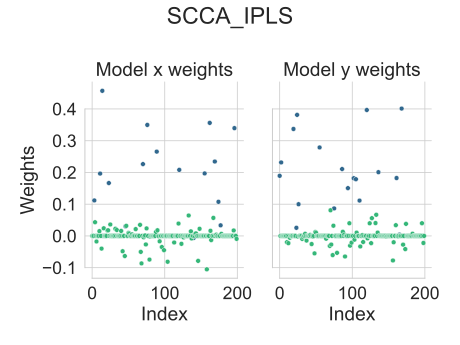
\includegraphics[width=0.6\textwidth]{figures/als/simulated/SCCA_IPLS_weights.svg}
    \caption{IPLS captures the true underlying signal effectively, thanks to its sparsity priors.}
    \label{fig:IPLS_weights}
\end{figure}

\paragraph{Advantage of Elastic Net:}
Elastic Net regularization combines both $l_1$ and $l_2$ penalties. As Figure~\ref{fig:ElasticNet_weights} shows, this strikes a good balance between feature selection and signal capture.

\begin{figure}[h]
    \centering
    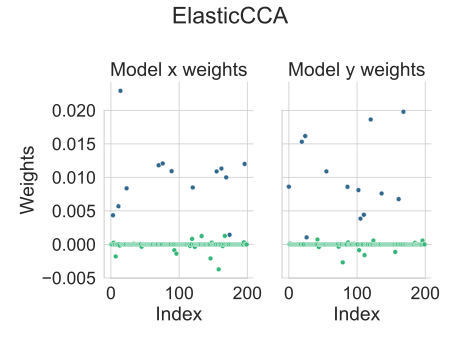
\includegraphics[width=0.6\textwidth]{figures/als/simulated/ElasticCCA_weights.svg}
    \caption{Elastic Net shows balanced feature selection and effective signal capture.}
    \label{fig:ElasticNet_weights}
\end{figure}

\paragraph{Superiority of IPLS+:}
As illustrated in Figure~\ref{fig:IPLS+_weights}, IPLS+ with a positive constraint shows the best performance among the models tested, emphasizing the benefit of domain-specific priors.

\begin{figure}[h]
    \centering
    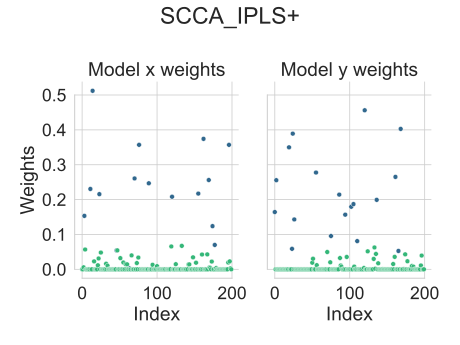
\includegraphics[width=0.6\textwidth]{figures/als/simulated/SCCA_IPLS_positive_weights.svg}
    \caption{IPLS+ outperforms other models, benefiting from a positive constraint.}
    \label{fig:IPLS+_weights}
\end{figure}

\subsection{Conclusion}

The experimental results underscore the importance of incorporating sparsity and other domain-specific priors in multiview learning models.
The interleaved figures and discussions affirm the need to align the model's objective with the characteristics of the underlying signal for effective feature selection and signal capture.




\subsection{Experiment 2: Human Connectome Project (HCP) Data Evaluation}

\subsubsection{Experiment Design}
In our study, we used resting-state fMRI along with non-imaging subject measures from a total of 1003 healthy subjects, sourced from the 1200-subject data release of the Human Connectome Project (HCP). The dataset was divided into an 80\% training set and a 20\% testing set.
To fine-tune the regularization of hyperparameters, cross-validation was employed within the training data.
Our approach, dubbed Flexible Regularized Alternating Least Squares (FRALS) with elastic net regularization on both views, was compared against existing methods, namely separate PCA on each modality, Penalized Matrix Decomposition (PMD), and Ridge Regularized CCA (RCCA). The performance was evaluated based on out-of-sample correlations.

\subsubsection{Performance Metrics}
The primary metric for evaluating the performance of our FRALS model was out-of-sample canonical correlations.
It was compared against PCA performed individually on each modality, as well as against PMD and RCCA\@.

\subsubsection{Performance Metrics}
Our model, FRALS, demonstrated superior performance by achieving the highest out-of-sample canonical correlations among all models tested (see Figure \ref{fig:performance}).

\begin{figure}[h]
\centering
\includesvg[width=0.5\linewidth]{figures/als/hcp/barcorr}
\caption{Out-of-sample canonical correlations for each model.}
\label{fig:performance}
\end{figure}

\subsubsection{Model Similarities}
We computed the correlation matrix of the scores for each modality to evaluate the similarity of the latent variables learned by each model. FRALS exhibited low or negative correlations with other models, highlighting its ability to capture novel and distinct aspects of brain-behaviour associations (see Figure \ref{fig:similarities}).

\begin{figure}[h]
\centering
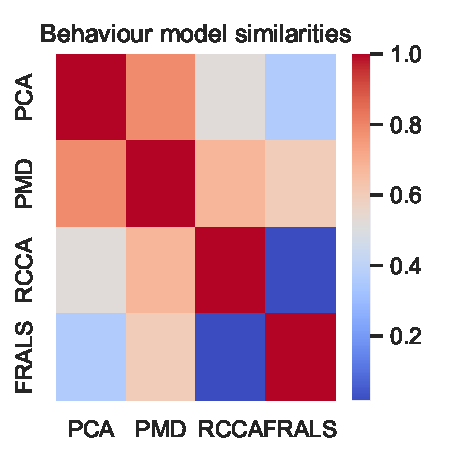
\includegraphics[width=0.49\linewidth]{figures/als/hcp/behaviour_model_similarities}
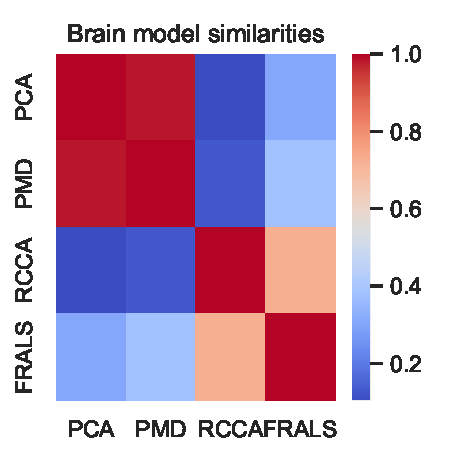
\includegraphics[width=0.49\linewidth]{figures/als/hcp/brain_model_similarities}
\caption{Left: Correlation matrix of the scores for each modality. Right: Correlation matrix of the brain loadings for each model.}
\label{fig:similarities}
\end{figure}


\subsubsection{Behaviour and Brain Loadings}
In terms of behavioral loadings, except for PCA, all models identified a latent variable that correlated positively with cognitive tests and negatively with cigarette, tobacco, or alcohol use.
Both RCCA and FRALS demonstrated stronger correlations with the Line Orientation test, which measures visuospatial abilities.

\begin{figure}[h]
\centering
\includesvg[width=\linewidth]{figures/als/hcp/all_top_and_bottom_loadings.svg}
\caption*{Top 5 positive and negative non-imaging loadings for each model}
\label{fig:behaviour}
\end{figure}

Regarding the brain loadings, our analysis shows that each model assigns different weights to various brain regions
based on their connectivity.
RCCA and FRALS assigned more weight to the parietal lobe, known for its role in visuospatial processing, than did PCA and PMD. This suggests that the parietal lobe is more relevant for the brain-behaviour correlations captured by our model.
Conversely, PMD appears to rely on principal components in the brain, potentially missing the true associations between the views.
FRALS functions as a sparse version of RCCA in this context.

\begin{figure}[h]
\centering
\includegraphics[width=0.49\linewidth]{figures/als/hcp/pca_brain_loadings.pdf}
\includegraphics[width=0.49\linewidth]{figures/als/hcp/pmd_brain_loadings.pdf}
\includegraphics[width=0.49\linewidth]{figures/als/hcp/rcca_brain_loadings.pdf}
\includegraphics[width=0.49\linewidth]{figures/als/hcp/flexals_brain_loadings.pdf}
\caption*{Map of CCA connection strength increases/decreases, with each node’s parcel map weighted by CCA edge-strength increases, summed across edges involving that node.}
\label{fig:brain}
\end{figure}

\section{Discussion}


\section{Limitations}\label{sec:limitations}

While FRALS offers promising performance in terms of out-of-sample correlation, it does come with significant drawbacks, the most noteworthy being its computational inefficiency. Below, we outline the primary factors contributing to the slow speed of FRALS and provide some insights into the computational bottlenecks.

\subsection{Computational Time}\label{subsec:computational-time}
One of the major constraints of FRALS is the time complexity involved in solving the regularized least squares regressions to completion. The algorithm’s iterative nature, which involves solving a sequence of regressions, makes it computationally intensive, particularly when dealing with high-dimensional data.

\subsection{Changing Regression Targets}\label{subsec:changing-regression-targets}
Adding to the computational burden is the fact that the regression targets, i.e., the projections of the other view, are not static but change dynamically throughout the algorithm's run.
Each update to the least squares solution consequently alters the global objective, leading to a constantly shifting landscape that the algorithm needs to navigate.





\subsection{Conclusions and Further Work}
The main idea of this chapter is to introduce FRALS, a novel approach in the realm of multiview learning that optimizes
both flexibility and performance.
Our experiments indicate that FRALS not only outperforms established methods like PCA, PMD, and RCCA in terms of out-of-sample canonical correlations but also captures novel and distinct aspects of brain-behavior associations.
This uniqueness is evident from the low or negative correlations FRALS holds with other models.

Our findings also underline the importance of the parietal lobe in understanding brain-behavior associations.
FRALS emphasizes this region more compared to traditional methods like PCA and PMD. Future work should focus on understanding the specific functions and contributions of different brain regions captured by FRALS and how they relate to various behaviors.

Given its promising initial results, the next step for FRALS would be its application to larger datasets and its adaptation for different kinds of biological and non-biological data to further evaluate its robustness and applicability.



\section{Conclusion}

We have introduced a flexible and efficient framework for regularized CCA that addresses the limitations of existing methods.
Our framework is particularly well-suited for high-dimensional data and can be adapted to various types of regularization, offering an effective tool for uncovering complex relationships in multiview data.







